\chapter{Pendahuluan}
Selalu ada aspek negatif dari sebuah pemanfaatan teknologi.
Teknologi informasi tidak lepas dari masalah ini.
Ada banyak manfaat dari teknologi informasi.
Sayangnya salah satu aspek negatifnya adalah masalah keamanan
({\em security}).

Banyak tulisan dan buku yang mengajarkan cara merusak sebuah
sistem informasi. Sementara itu buku yang mengajarkan cara
pengamanannya agak minim. Demikian pula, ilmu untuk mengamankan
sistem berbasis teknologi informasi juga harus lebih banyak
diajarkan.

%%%
\section{Keamanan Informasi}
Ketika kita berbicara tentang {\em security}, yang muncul dalam
benak kebanyakan orang adalah {\em network security}, keamanan jaringan.
Padahal sesungguhnya yang ingin kita amankan adalah \textbf{informasi}.
Bahwa informasi tersebut dikirimkan melalui jaringan adalah benar,
tetapi tetap yang ingin kita amankan adalah informasinya.
Nanti akan kita bahas lebih lanjut mengapa demikian.
Maka judul dari buku ini adalah ``Keamanan Informasi''.

%%%
\section{Beberapa Contoh Kasus}
Untuk menunjukkan betapa banyaknya masalah keamanan informasi,
berikut ini ada beberapa contoh kasus-kasus.
Contoh ini bukanlah daftar yang komplit, melainkan hanya sampel
dari kondisi yang ada. Bahkan, kemungkinan kondisi yang ada
lebih parah daripada contoh-contoh ini.

Beberapa contoh kasus di luar negeri (diurutkan berdasarkan
tahun kejadiannya) antara lain dapat dilihat dari daftar berikut.

\begin{enumerate}
\item 2006-2008. Tahun-tahun ini ditandai dengan mulai masuknya
   aspek manajemen ke dalam bidang keamanan informasi.
   Standar ISO (mulai dari 17799 dan kemudian menjadi seri 27000)
   mulai digunakan di berbagai instansi.
   Adanya bencana alam (tsunami, banjir, gempa, dan sejenisnya)
   membuat orang mulai memikirkan keberlangsungannya sistem IT.
   Perangkat IT semakin mengecil dalam ukuran sehingga mulai dibawa
   pengguna ke kantor. Misalnya pengguna membawa sendiri akses
   internet dengan menggunakan handphone 3G.
   Penggunaan kartu sebagai pengganti uang juga mulai populer.
   (Less cash society.)

\item 2013. Virus masih tetap mendominasi masalah.
   Pencurian identitas ({\em identity theft}) mulai marak.
   Cyber war mulai menjadi bagian dari diskusi.
\item 2014. Heartbleed dan Bash Bug.
   (Yang ini lebih mudah dijelaskan dengan menggunakan gambar.
   Sayangnya saya tidak memiliki hak untuk memasukkan gambar tersebut
   ke dalam buku ini. Di kesempatan berikutnya akan saya usahakan
   memberi penjelasan dengan kata-kata dulu.)
\item 2014. Bursa Singapura terganggu karena masalah software.
   Perdagangan saham sempat terhenti.
\item 2016.
   Sebuah firma hukum di Panama bernama Mossack Fonseca (MF)
   mengalami kebocoran data.
   Data yang bocor berupa tabungan / investasi orang-orang terkenal
   dari beberapa negara (termasuk Indonesia).
   Kasus ini disebut {\em Panama Papers Breach}.
   Kebocoran ini diduga karena {\em Slider plugin} yang digunakan
   oleh situsnya (yang menggunakan Wordpress) sudah kadaluawarsa dan
   memiliki kerentanan. Hasil eksploitasi memperkenankan orang untuk
   mengambil berkas sesukanya.
\item 2016. 
   CCTV digunakan sebagai bagian dari Distributed DoS attack.
   Ini menunjukkan bahwa perangkat yang menjadi bagian dari
   Internet of Things (IoT) dapat menjadi target serangan
   untuk kemudian dijadikan ``anak buah'' (zombie) untuk
   menyerang tempat lain.
   Kode sumber Mirai yang digunakan untuk melakukan penyerangan
   tersedia di internet. Jika kita tidak siap, ini dapat menjadi
   masalah yang berikutnya.
\item 2016.
   Serangan DDoS terhadap berbagai DNS (Domain Name System) servers.
   Serangan menggunakan bantuan {\em botnet}
   sehingga menghabiskan {\em bandiwdth} jaringan dalam orde
   Gbps.
\end{enumerate}

Selain contoh-contoh di atas, tentunya masih banyak kasus-kasus lain.
Ada yang menganalogikan ini sebagai puncak dari {\em iceberg}.
Di bawah laut lebih banyak lagi masalah yang tidak terlihat.

Beberapa contoh kasus yang terkait dengan Indonesia dapat
dilihat dari daftar berikut.

\begin{enumerate}
\item 1999. Nama domain Timor Timur (.TP) diacak-acak.
   Diduga pelakunya adalah pemerintah Indonesia.
   Investigasi lebih lanjut menunjukkan bahwa ini tidak dilakukan
   oleh pemerintah Indonesia tetapi oleh seseorang (atau sekelompok)
   yang berada di Amerika Serikat.
\item 2011. Perusahaan Research in Motion (RIM) yang memproduksi
   {\em Blackberry} dipaksa untuk memiliki server di Indonesia.
   Alasan utama adalah agar dapat dilakukan {\em lawful interception},
   yaitu penyadapan secara legal untuk kasus-kasus tertentu.
   Pihak RIM keberatan. Tidak ada server RIM di Indonesia.
\item 2015. Serangan man-in-the-browser (MITB) dilakukan terhadap
   berbagai layanan internet banking di Indonesia sehingga mengakibatkan
   hilangnya uang nasabah\footnote{http://regional.kompas.com/read/
   2015/08/11/12185971/
   Kronologi. Hilangnya. Uang. Nasabah. Bank. Mandiri.
   Versi. Korban}
\item 2016. Aplikasi Pokemon Go mulai muncul dan ramai digunakan.
   Aplikasi ini menggunakan lokasi pengguna sebagai bagian dari
   permainannya, yaitu untuk menampilkan monster Pokemon sesuai
   dengan lokasi.
   Selain itu, foto dari lingkungan sekitarnya dapat juga kita ambil
   dan kita bagikan (share) dengan orang lain melalui media sosial.
   Aplikasi ini dilarang digunakan di lingkungan milter dan
   pemerintahan karena dikhawatirkan dapat membocorkan data rahasia.
   (Sebetulnya ada banyak aplikasi lain yang juga menggunakan data
   lokasi seperti {\em Waze} dan {\em Google Maps}, tetapi ini tidak
   ``terlihat''. Bahkan lebih berbahaya lagi adalah penggunaan
   layanan email gratisan untuk akun resmi pemerintahan atau instansi
   lain di Indonesia.)
\item 2016.
   Berbagai {\em market place} (seperti Tokopedia, Bukalapak, dll.)
   dan aplikasi handphone (seperti Go-Jek) diserang oleh orang
   yang mencoba melakukan password cracking.
   Asumsinya adalah seseorang akan menggunakan userid (alamat email)
   dan password yang sama untuk situs-situs tersebut.
   Identitas yang bocor di sebuah layanan (web site, application)
   dicoba digunakan di tempat lain. 
\item 2016. Topik pembentukan ``Badan Cyber Nasional (BCN)''
   mulai hangat dibicarakan.
\end{enumerate}

Saat ini semakin banyak lagi masalah keamanan yang ditemui.
Hal ini disebabkan semakin banyak pemanfaatan teknologi informasi dan
jaringan internet.
Selain itu teknik untuk menemukan lubang keamanan juga semakin
canggih sehingga lebih banyak ditemukan kelemahan-kelemahan tersebut.

Sebuah survey yang dilakukan oleh {\em Information Week} di Amerika
Serikat (tahun?) menunjukkan bahwa hanya 22 persen manager yang
menganggap keamanan sistem informasi sebagai hal yang penting.
Bagaimana meyakinkan mereka untuk melakukan investasi di pengamanan?

Rendahnya kesadaran atas masalah keamanan (lack of security awareness)
merupakan salah satu kunci utama munculnya masalah keamanan.
Para praktisi juga masih menjalankan kebiasaan buruk,
seperti misalnya berbagi password admin.

Masalah keamanan informasi yang biasanya berupada data teknis
harus diterjemahkan ke angka finansial agar dapat dimengerti 
oleh pihak pimpinan.
Sebagai contoh, di Inggris ada survey mengenai berapa biaya
yang dikeluarkan perusahaan jika sistem mereka tidak dapat
diakses ({\em down}).



\section{Security Life Cycle}
Banyak orang yang beranggapan bahwa masalah keamanan informasi
dapat dipecahkan dengan membeli produk keamanan,
misalnya firewall, anti-virus, dan seterusnya.
Kemanan informasi sebetulnya berupa sebuah siklus
sebagaimana ditampilkan pada Gambar~\ref{fig:security-life-cycle}.

\begin{figure}[ht]
\fbox{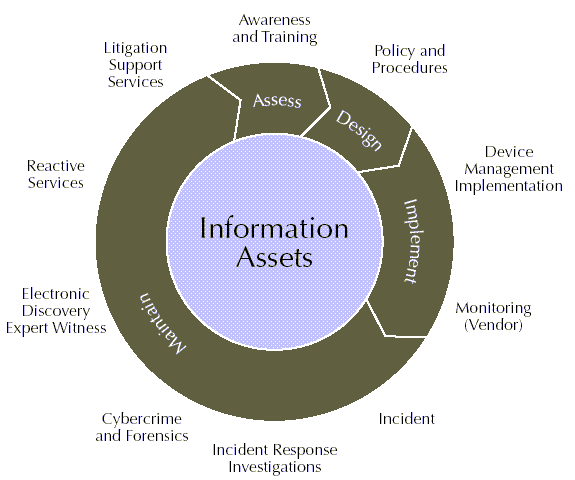
\includegraphics[width=1.0\linewidth]{graphics/security-life-cycle.png}}
\caption{Security Life Cycle}
\label{fig:security-life-cycle}
\end{figure}
